\documentclass[../report.tex]{subfiles}
\begin{document}
\section{Essential Behaviours to Solve the Sokoban Game} \label{sec:behaviours}

The Sokoban game has a set of rules, which the build robot must follow to not get disqualify from the game. Therefore, a set of behaviours must be incubated in the control design of the robot to make it solve the puzzle correctly.

To make the environment easy for the robot to interact with, the robot is only told to go from intersection to intersection. The idea is to create a sequence of simple tasks which the robot solves one by one. The sequence is made by the sokoban solver and will be explained further in section \ref{subsec:sokoban_solver}. The sequence will consist of task described in table \ref{tab:behaviours}.

\begin{table}[H]
\centering
\begin{tabular}{lll}
\toprule
\textbf{Number} & \textbf{Name} & \textbf{Description} \\ \midrule
1 & Follow & Follow a line. \\
2 & Intersection & Detect an intersection. \\
3 & Forward & Run forward for a certain period. \\
4 & Backwards & Run backwards for a certain period. \\
5 & Turn left & Rotate left for a certain period. \\
6 & Turn right & Rotate right for a certain period. \\
7 & Turn 180 & Perform two right turns (6) in a row. \\ \bottomrule
\end{tabular}
\caption{Behaviours for the robot to solve the sokoban puzzle.}
\label{tab:behaviours}
\end{table}

% Firstly, the robot must be able to move around the map. Therefore, two large motors are implemented on the robot. Thereby, making the robot able to control two wheels separately. Thus, the robot is able to turn and move on the map. The mounted large motors are shown on figure \ref{fig:robot_design}.
% \begin{figure}[H]
%     \centering
%     \begin{subfigure}[t]{0.5\textwidth}
%         \centering
%         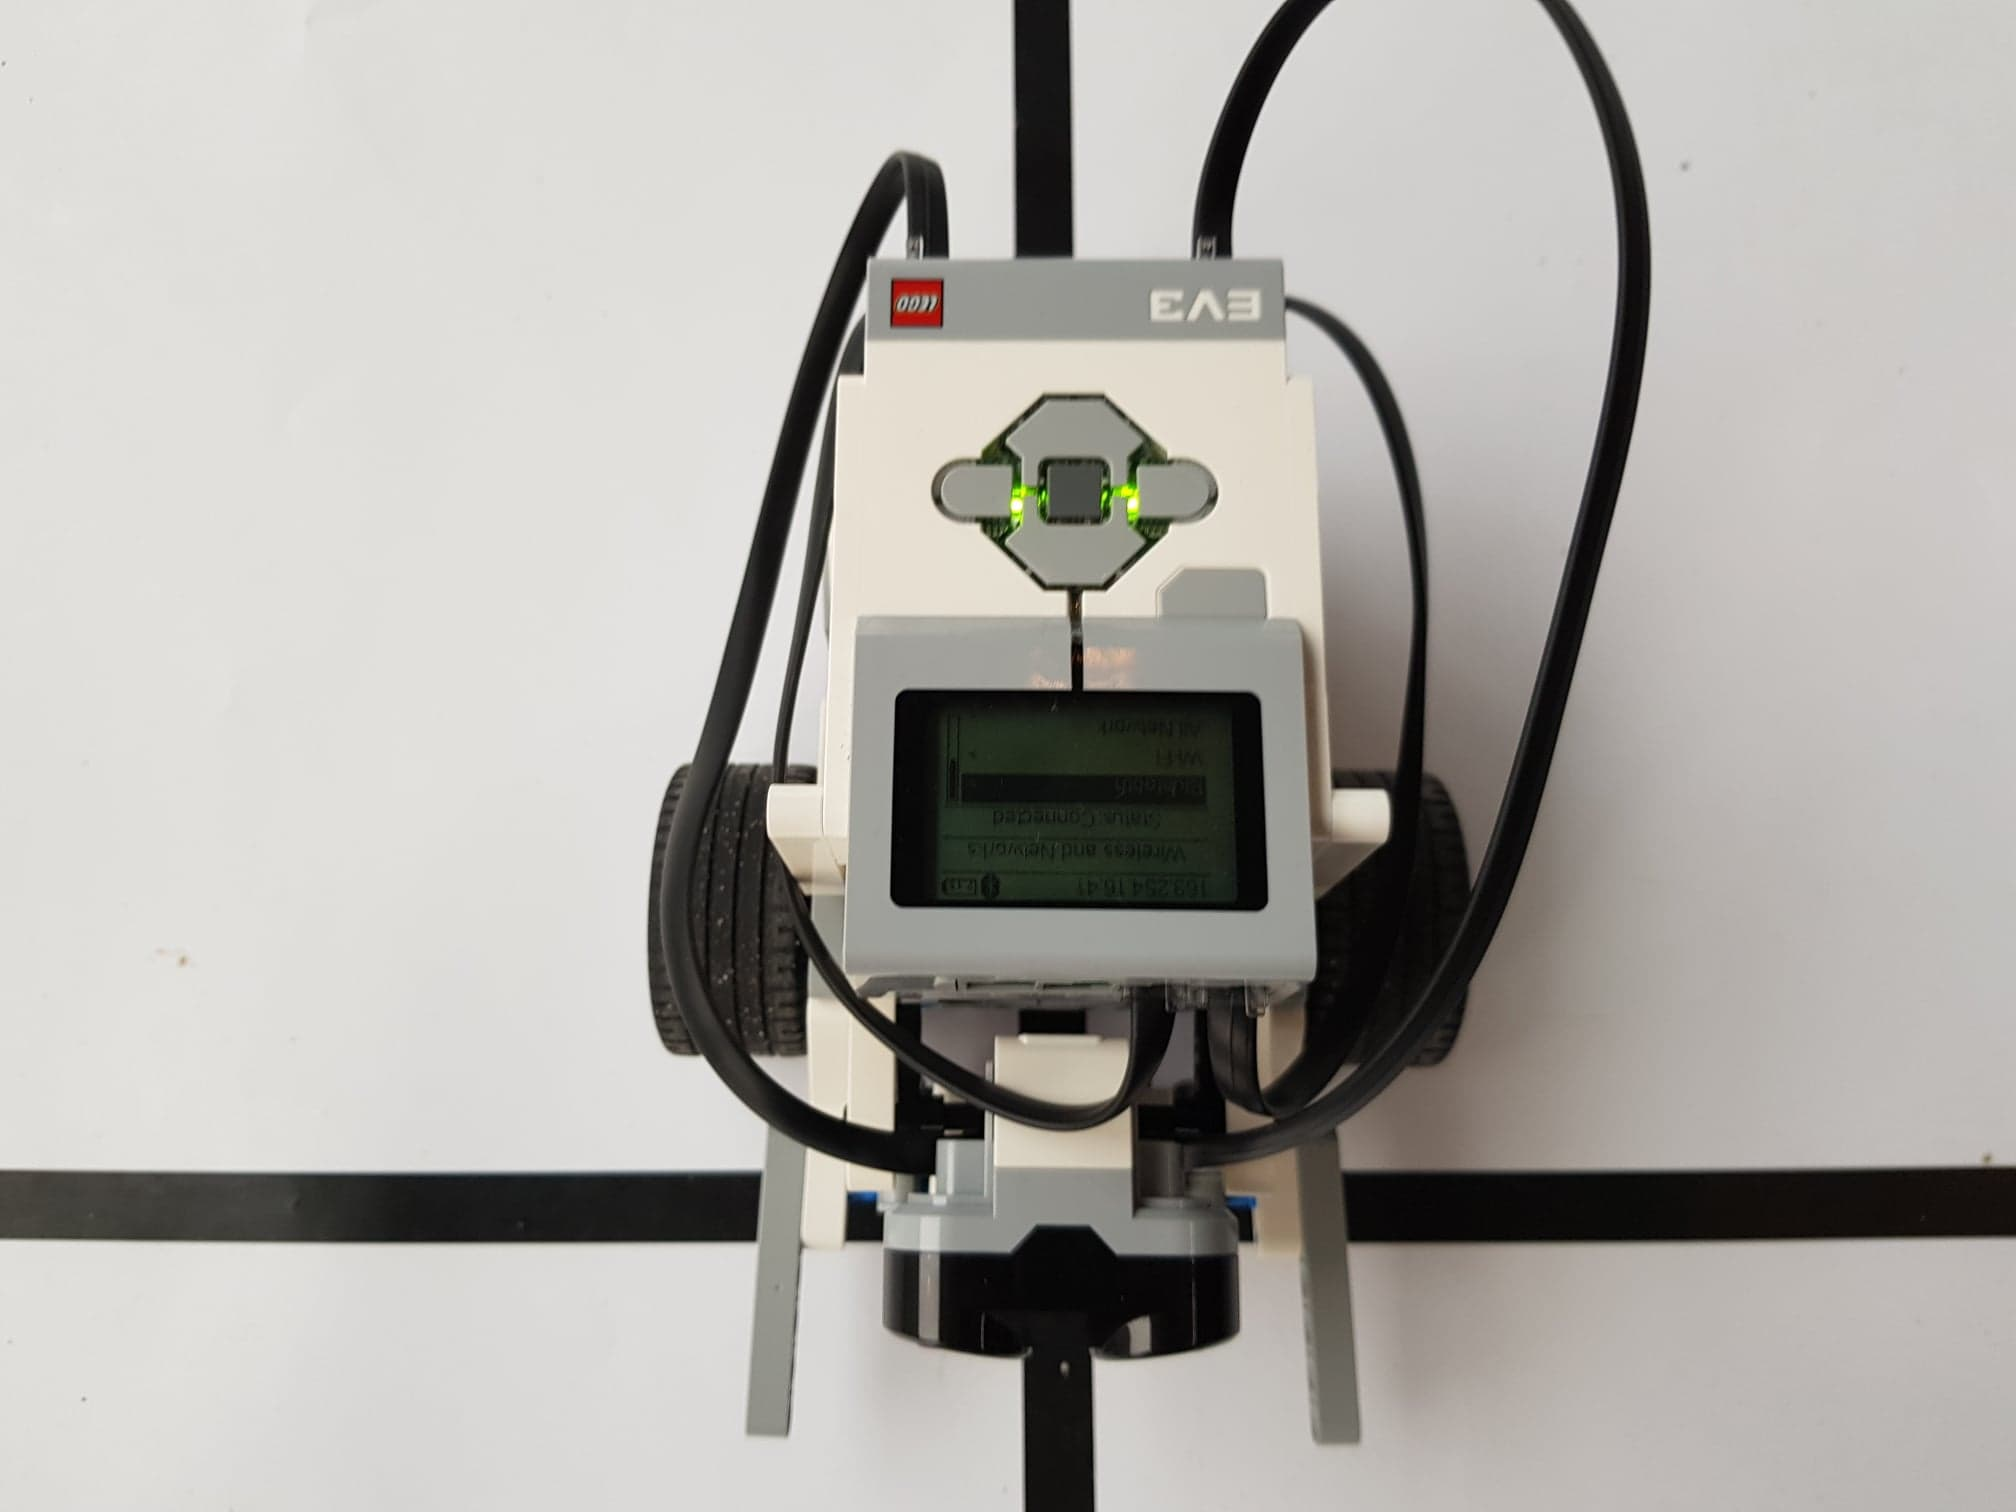
\includegraphics[width=0.9\textwidth]{figures/robot_design/color_sensor_intersection.jpg}
%         \caption{Top view of robot design at intersection.}
%         \label{fig:color_sensors_intersection}
%     \end{subfigure}%
%     \begin{subfigure}[t]{0.5\textwidth}
%         \centering
%         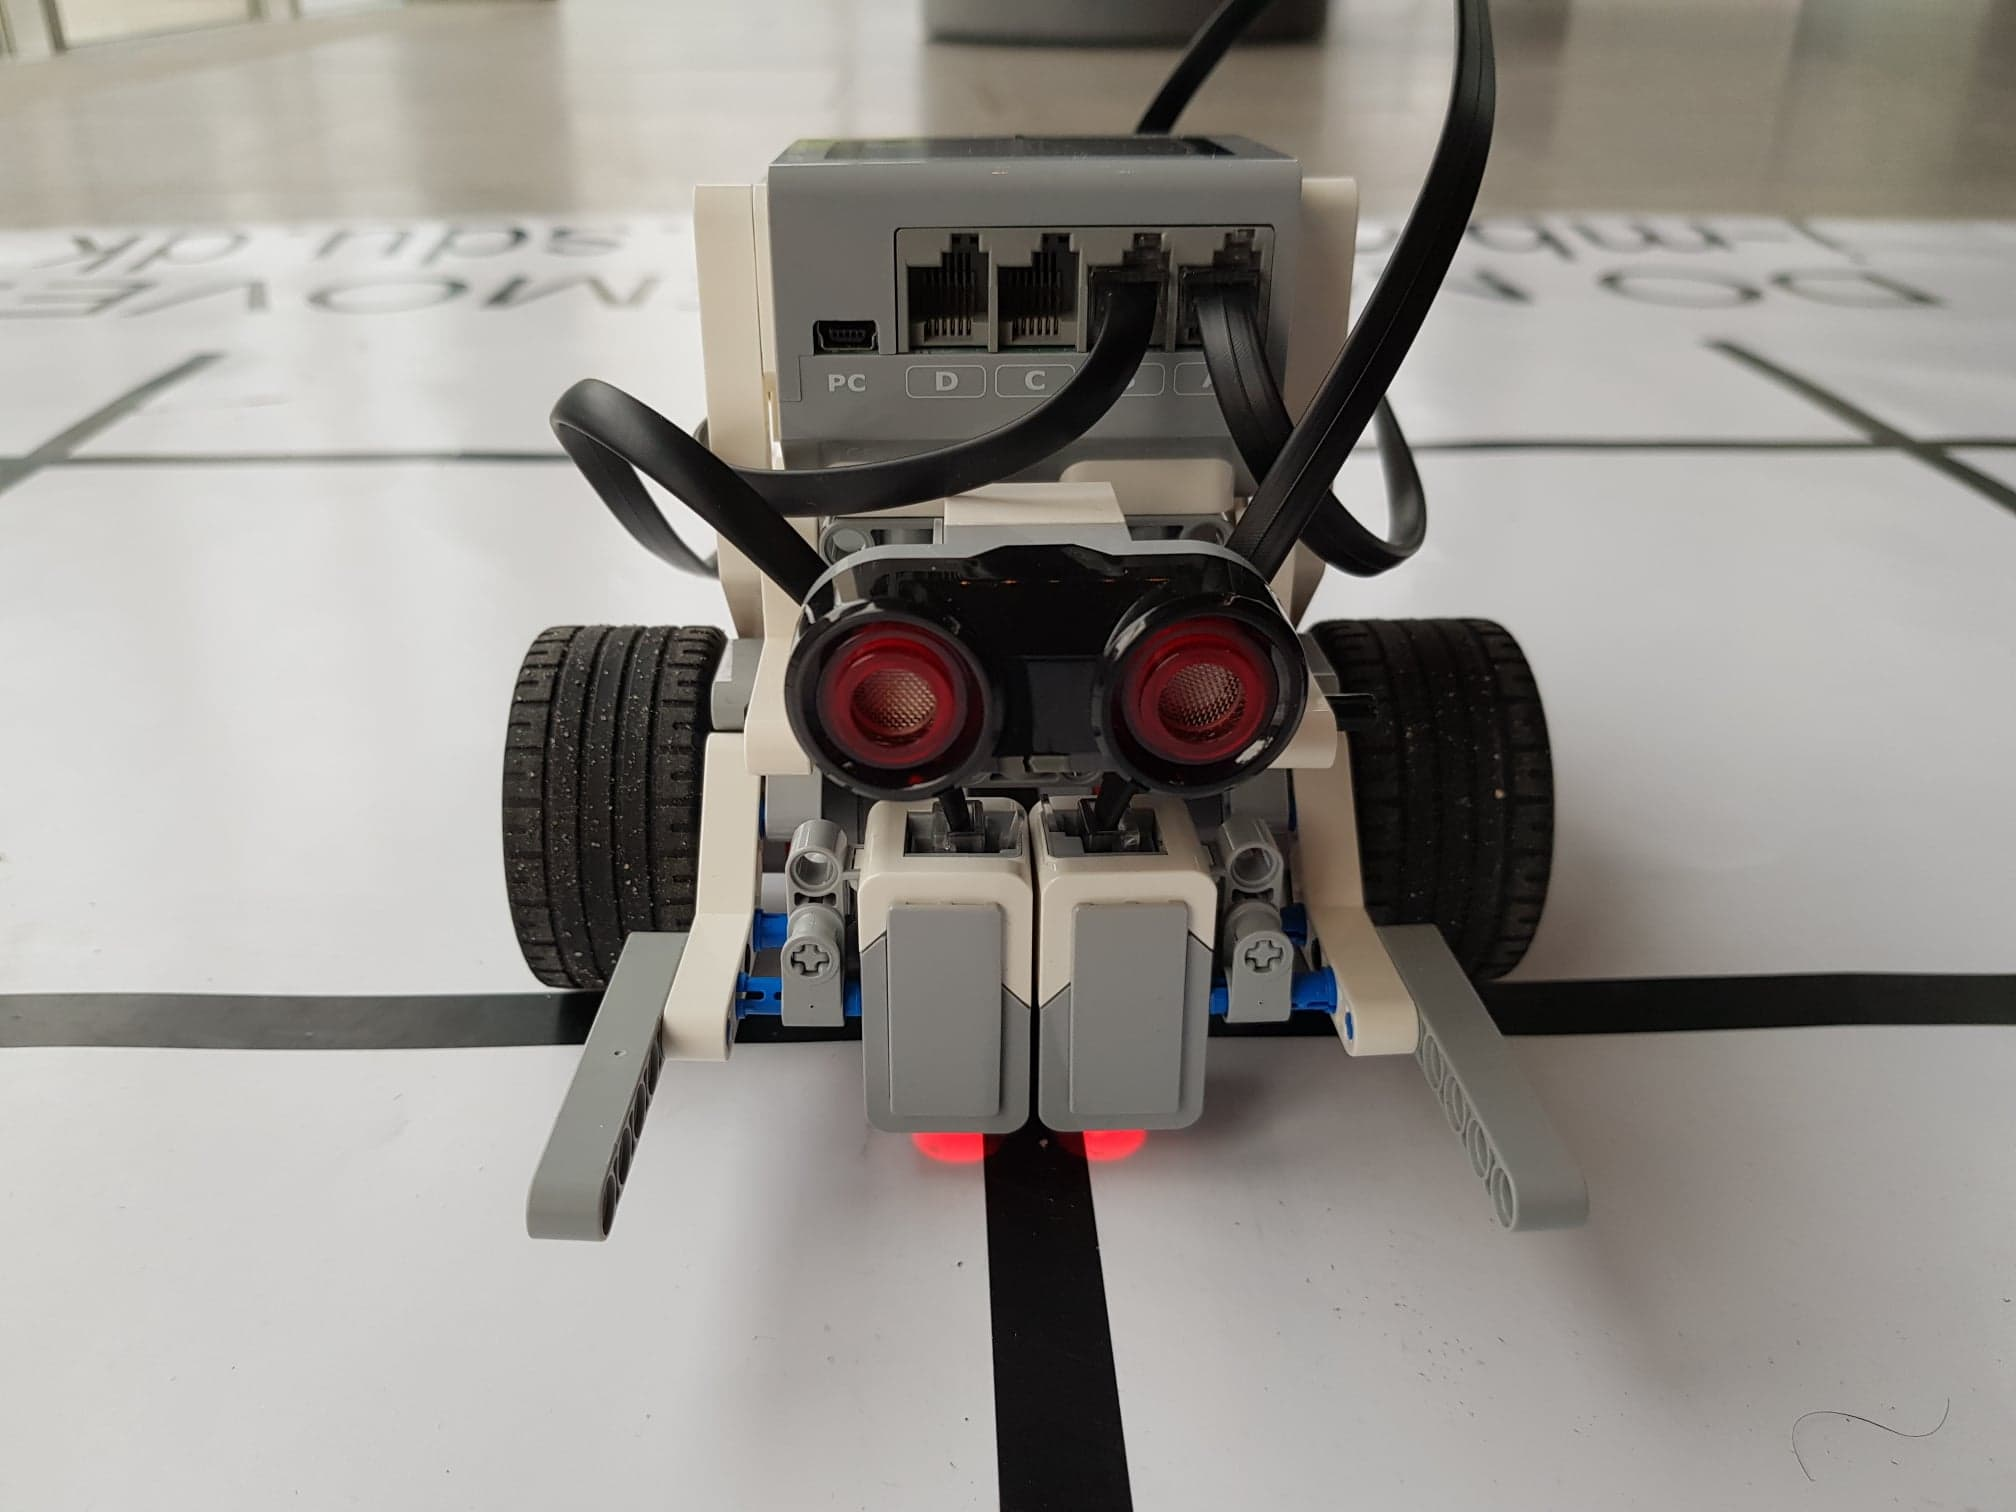
\includegraphics[width=0.9\textwidth]{figures/robot_design/color_sensor_linefollower.jpg}
%         \caption{Front view of robot design when following a line.}
%         \label{fig:color_sensors_line_follower}
%     \end{subfigure}
%     \caption{Views of the constructed robot design.}
%     \label{fig:robot_design}
% \end{figure}
% The map is build up by lines, which the robot has to follow, as illustrated in figure \ref{fig:sokoban_map}. Therefore, a needed behaviour is to follow a line. To control this behaviour two color sensors are used. The sensors are mounted as shown in figure \ref{fig:color_sensors_front_view}. The line follower behavior is constructed as a reactive controller. Thus, the color sensors are connected to the large motor mounted at the same side. 
% The lines on the map intersects, as illustrated in figure \ref{fig:sokoban_map}. Therefore the robot must be able to detect intersection. This is necessary because of two main reasons: to know where the robot is in the environment by using the intersections as landmarks and to use the intersection as points where the robot can drive forward, backward, left and right until a new intersection is reached. The two color sensors are used to detect intersection, by measuring when both the sensors have a low intensity.
\end{document}